\documentclass[12pt, a4paper]{article}
\usepackage{amsmath}
\usepackage{amsfonts}
\usepackage{amsthm}
\usepackage{mathtools}
\newtheorem{theorem}{Theorem}[section]
\newtheorem{definition}{Definition}[section]
\numberwithin{equation}{section}
\usepackage{pgfplots}
\pgfplotsset{width=10cm,compat=1.9}
\graphicspath{ {img/} }
\DeclareGraphicsExtensions{.png, .jpg}

\title{Ensemble methods}
\author{Kristian Wichmann}

\begin{document}
\maketitle

\textit{Ensemble learning} in machine learning is broadly speaking the practice of making a collection - an \textit{ensemble} - of models, and combine them into a single model with more desired properties.

\section{Bagging and boosting}
There are two broad categories of such meta-algorithms:

\subsection{Bagging}
\textit{Bagging} is short for \textit{bootstrap aggregation}. This is because the ensembles are made through bootstrapping, i.e. random resampling from the training set. Properties of these meta-algorithms:

\begin{itemize}
\item Ensembles are build independently in \textit{parallel}.
\item Tends to reduce variance.
\end{itemize}

\subsection{Boosting}
Properties of these meta-algorithms:
\begin{itemize}
\item Ensembles are build \textit{sequentially}, each building on the ones before.
\item Tends to reduce bias.
\end{itemize}

\section{Simple, unweighted boosting}
As noted above, the general idea behind boosting is to combine an ensemble of weak learners into one strong learner. Here, the term \textit{weak learner} means one that is slightly better than random guessing.

\subsection{Wisdom of the crowd}
The most basic type of boosting is known from the quiz show "Who wants to be a Millionaire?". One of the lifelines is asking the audience. Here, a simple majority vote determines what is usually the best answer. This phenomenon is also known as the \textit{wisdom of the crowd}.

The procedure above describes a classification problem. For regression type problems, the mean of the individual predictions would be used instead of majority vote.

\subsection{Example: Binary classification with three learners}
As a simple example consider three binary classifiers $h_1, h_2, h_3$ on a training set $X$. The two classes corresponds to values of $\pm 1$. The true labels are denoted $f(x)$. Then the simple boosting classifier as described above can be written like:
\begin{equation}
H(x)=\textrm{sgn}\left[h_1(x)+h_2(x)+h_3(x)\right]
\label{simple_three_boost}
\end{equation} 

\begin{figure}
\centering
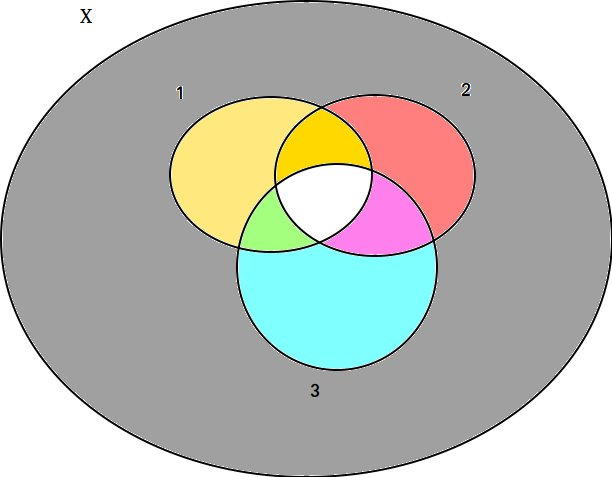
\includegraphics[width=0.6\textwidth]{three_unweighted}
\caption{Regions of error for the binary classification with three learners.}
\label{fig:three_unweighted}
\end{figure}

The situation is visualized in figure \ref{fig:three_unweighted}. Each of the three initial classifiers has a region in which its prediction is wrong. These are shown as the regions 1, 2, and 3 respectively. The boosted classifier is only wrong when two or all of the three initial classifiers are wrong. In other words, the error region for $H$ consists of the union of the four regions in orange, green, purple, and white.

Now, initially this looks like an improvement, but in fact in needs not be! Imagine that there's one data point in each of the four regions mentioned above, and none in the yellow, red and blue ones. Then each of $h_1, h_2$, and $h_3$ misclassify three points, while $H$ actually misclassifies four!

\section{AdaBoost}
As the example above shows, we need to be more clever to ensure a good boosting strategy. \textit{AdaBoost}, which is short for \textit{adaptive boosting} is one such widely used algorithm.

\subsection{Weighted binary classification}
Consider equation \ref{simple_three_boost}, but for $T$ learner instead of three. We can generalize this by including \textit{weights} for each classifier:
\begin{equation}
H(x)=\textrm{sgn}\left[\sum_{t=1}^T \alpha_t h_t(x)\right]
\end{equation}
This introduces more flexibility - more \textit{capacity} - to our boosted model. The question now of course is both how to create the classifiers $h_t$ and how to pick the weights $\alpha_t$ appropriately.

\subsection{The base algorithm}
To build our weak learners, we must use some \textit{base algorithm}, which we will denote $\mathcal{L}$ for short. The only requirement is, that for a given probability distribution $D$ on the training set $X$, we can build a classifier:
\begin{equation}
\mathcal{L}[X,D]
\end{equation}

\end{document}